\documentclass[11pt,a4paper]{article}
\usepackage[margin=21mm,top=19mm,bottom=19mm]{geometry}
\usepackage{fontspec,xeCJK,amsmath,amssymb,booktabs,array,graphicx,float,caption,titlesec,fancyhdr}
\usepackage[hidelinks]{hyperref}
\hypersetup{pdftitle={模型融合保护方法研究进展},pdfsubject={防御二：基于任务子空间的全网络通道置换；防御一：视觉投影零空间中的偏置扰动}}
\setmainfont{Times New Roman}
\setCJKmainfont{SimSun}[AutoFakeBold=1.6]
\setCJKsansfont{SimSun}[AutoFakeBold=1.6]
\XeTeXlinebreaklocale "zh"
\XeTeXlinebreakskip=0pt plus 1pt
\linespread{1.16}
\setlength{\parindent}{2em}
\setlength{\parskip}{3pt}
\setlength{\tabcolsep}{5pt}
\renewcommand{\arraystretch}{1.18}
\renewcommand{\figurename}{图}
\renewcommand{\tablename}{表}
\renewcommand{\refname}{参考文献}
\captionsetup{font=small,labelfont=bf,labelsep=quad,skip=6pt}
\titleformat{\section}{\large\bfseries}{\thesection}{.65em}{}
\titleformat{\subsection}{\normalsize\bfseries}{\thesubsection}{.6em}{}
\titlespacing*{\section}{0pt}{11pt}{7pt}
\titlespacing*{\subsection}{0pt}{7pt}{3pt}
\pagestyle{fancy}\fancyhf{}
\fancyhead[L]{\small 模型融合保护方法研究进展}
\fancyhead[R]{\small 2026年10月23日}
\fancyfoot[C]{\small\thepage}
\renewcommand{\headrulewidth}{.35pt}
\setlength{\headheight}{14pt}
\newcommand{\tabnote}[1]{\par\vspace{4pt}\begin{minipage}{.98\linewidth}\footnotesize #1\end{minipage}}
\newcommand{\norm}[1]{\left\lVert#1\right\rVert}
\newcommand{\reporttablesettings}{%
\begin{table}[H]
\centering
\small
\caption{任务与评价规模}\label{tab:settings}
\begin{tabular}{@{}llrr@{}}
\toprule
数据集 & 任务 & 类别数 & 完整测试样本数 \\
\midrule
MNIST & 手写数字 & 10 & 10,000 \\
DTD & 纹理分类 & 47 & 1,880 \\
SVHN & 街景数字 & 10 & 26,032 \\
\bottomrule
\end{tabular}

\end{table}
}


\newcommand{\reporttablemain}{%
\begin{table}[H]
\centering
\footnotesize
\caption{双专家主实验：TA系数为0.5，准确率（\%）}\label{tab:main}
\begin{tabular}{@{}llrrrr@{}}
\toprule
保护任务 / 伙伴 & 方法 & 独立使用 & 直接融合 & \shortstack{AGA\\仅保护专家} & \shortstack{AGA\\双方专家} \\
\midrule
MNIST / SVHN & 无保护 & 99.69 & 99.37 / 92.50 & 99.30 / 92.78 & 99.32 / 91.77 \\
MNIST / SVHN & PaRaMS & 99.69 & 8.92 / 9.15 & 99.30 / 92.79 & 99.32 / 91.77 \\
MNIST / SVHN & 防御二 & 99.69 & 10.98 / 14.32 & 9.80 / 9.81 & 9.80 / 9.83 \\
MNIST / SVHN & 防御一 & 99.69 & 9.80 / 6.70 & 9.80 / 6.70 & 9.80 / 6.70 \\
\midrule
DTD / MNIST & 无保护 & 79.41 & 69.31 / 99.45 & 68.40 / 99.45 & 68.78 / 99.42 \\
DTD / MNIST & PaRaMS & 79.41 & 2.07 / 8.92 & 68.35 / 99.45 & 68.78 / 99.42 \\
DTD / MNIST & 防御二 & 79.41 & 2.39 / 10.29 & 2.39 / 10.09 & 2.39 / 10.09 \\
DTD / MNIST & 防御一 & 79.41 & 2.13 / 21.09 & 2.13 / 21.09 & 2.13 / 21.05 \\
\midrule
SVHN / MNIST & 无保护 & 97.46 & 92.50 / 99.37 & 91.56 / 99.39 & 91.77 / 99.32 \\
SVHN / MNIST & PaRaMS & 97.46 & 9.09 / 8.95 & 91.56 / 99.39 & 91.77 / 99.32 \\
SVHN / MNIST & 防御二 & 97.46 & 7.30 / 9.45 & 6.45 / 12.19 & 6.45 / 12.22 \\
SVHN / MNIST & 防御一 & 97.46 & 6.70 / 9.80 & 6.70 / 9.80 & 6.70 / 9.80 \\
\bottomrule
\end{tabular}
\tabnote{融合列均为“保护任务 / 伙伴任务”；独立列只列保护任务。每种恢复方式分别使用其对应的无保护结果。PaRaMS使用完整官方默认配置。}
\end{table}
}


\newcommand{\reporttablecross}{%
\begin{table}[H]
\centering\footnotesize
\caption{其余三组保护方向的完整结果，准确率（\%）}\label{tab:cross}
\begin{tabular}{@{}llrrr@{}}
\toprule
保护任务 / 伙伴 & 方法 & 直接融合 & AGA仅保护专家 & AGA双方专家 \\
\midrule
MNIST / DTD & 无保护 & 99.45 / 69.31 & 99.43 / 69.41 & 99.42 / 68.78 \\
MNIST / DTD & 防御二 & 5.01 / 1.81 & 9.80 / 2.18 & 9.80 / 2.18 \\
\midrule
DTD / SVHN & 无保护 & 70.59 / 95.36 & 69.15 / 95.44 & 69.52 / 94.18 \\
DTD / SVHN & 防御二 & 2.93 / 8.85 & 2.34 / 6.42 & 2.34 / 6.42 \\
\midrule
SVHN / DTD & 无保护 & 95.36 / 70.59 & 94.09 / 70.74 & 94.18 / 69.52 \\
SVHN / DTD & 防御二 & 7.22 / 2.13 & 6.53 / 2.07 & 6.51 / 2.07 \\
\bottomrule
\end{tabular}
\tabnote{每格为“保护任务 / 伙伴任务”。与主表合计六个保护方向，对应三个无序任务组合。}
\end{table}
}

\newcommand{\reporttableablation}{%
\begin{table}[H]
\centering
\footnotesize
\caption{任务方向项的消融：保护任务准确率（\%）}\label{tab:ablation}
\begin{tabular}{@{}llrrrr@{}}
\toprule
保护任务 / 伙伴 & 选择目标 & 独立使用 & 直接融合 & AGA仅目标 & AGA双方 \\
\midrule
MNIST / SVHN & 任务方向与距离 & 99.69 & 10.98 & 9.80 & 9.80 \\
MNIST / SVHN & 仅距离 & 99.69 & 13.99 & 11.27 & 11.08 \\
\midrule
DTD / MNIST & 任务方向与距离 & 79.41 & 2.39 & 2.39 & 2.39 \\
DTD / MNIST & 仅距离 & 79.41 & 1.44 & 2.02 & 1.97 \\
\midrule
SVHN / MNIST & 任务方向与距离 & 97.46 & 7.30 & 6.45 & 6.45 \\
SVHN / MNIST & 仅距离 & 97.46 & 9.36 & 8.52 & 8.48 \\
\bottomrule
\end{tabular}
\tabnote{同一贪心规则、74个矩阵、32个任务奇异方向和384对交换。只改变构造目标；各目标的原始结果均保留。}
\end{table}
}


\newcommand{\reporttableeight}{%
\begin{table}[H]
\centering
\small
\caption{八专家融合：TA系数为0.2，保护任务准确率（\%）}\label{tab:eight}
\begin{tabular}{@{}lrrrr@{}}
\toprule
保护任务 & 无保护TA & 防御二TA & 无保护+AGA & 防御二+AGA \\
\midrule
MNIST & 94.00 & 10.26 & 93.23 & 11.35 \\
DTD & 52.18 & 3.24 & 51.38 & 4.89 \\
SVHN & 74.42 & 13.28 & 72.53 & 11.64 \\
\bottomrule
\end{tabular}
\tabnote{AGA只处理保护专家。八个专家参与合并，但只评价MNIST、DTD、SVHN，不报告八数据集平均。}
\end{table}
}


\newcommand{\reporttablesupplement}{%
\begin{table}[H]
\centering
\small
\caption{防御一的融合方法补充：原版AGA仅处理保护专家}\label{tab:supplement}
\begin{tabular}{@{}lrr@{}}
\toprule
融合方法 & 无保护 & 防御一 \\
\midrule
TA & 99.30 / 92.78 & 9.80 / 6.70 \\
TIES & 99.32 / 94.81 & 9.82 / 9.69 \\
DARE+TA & 99.30 $\pm$ 0.00 / 92.81 $\pm$ 0.04 & 24.20 $\pm$ 5.60 / 25.50 $\pm$ 10.30 \\
NUFILT：MNIST先 & 99.39 / 94.68 & 99.39 / 94.68 \\
NUFILT：SVHN先 & 99.07 / 95.35 & 99.07 / 95.35 \\
ProDistill & 99.42 / 96.83 & 9.80 / 6.70 \\
\bottomrule
\end{tabular}
\tabnote{每格为MNIST / SVHN准确率（\%）。DARE+TA为种子42、43、44的均值$\pm$样本标准差；各项使用匹配的无保护结果。ProDistill为使用无标签校准图的两专家适配。}
\end{table}
}

\begin{document}
\thispagestyle{plain}
\begin{center}
{\LARGE\bfseries 模型融合保护方法研究进展\par}
\vspace{7pt}
{\normalsize 2026年10月23日\par}
\end{center}
\vspace{2pt}
\section{研究问题与实验设置}
目标是在不重新训练原专家的条件下处理其参数：发布模型单独使用时仍能完成原任务，未经授权与其他专家融合后，受保护任务的准确率显著下降。设公开基座、目标专家、伙伴专家和发布模型分别为$\theta_0,\theta_e,\theta_p,\widetilde\theta_e$。独立能力与融合保护分别通过完整测试集评价，不以参数距离代替准确率。

主实验采用Task Arithmetic（TA）\cite{ta}：
\begin{equation}
\theta_{\mathrm m}=\theta_0+\lambda\big[(\widetilde\theta_e-\theta_0)+(\theta_p-\theta_0)\big],
\qquad\lambda=0.5.
\end{equation}
双专家情形因此等于两份专家参数的平均。所有方法使用相同的CLIP ViT-B/32骨干、分类头和完整测试划分。
\reporttablesettings

原版AGA\cite{aga}可以访问发布模型和公开基座，不预先知道所用防御。评价分为三列：直接融合；只恢复保护专家后融合；对双方专家分别恢复后融合。AGA源码固定在作者仓库的\texttt{fb61429}提交，没有针对本方法改写恢复过程。PaRaMS\cite{params}使用完整官方默认实现作为防御基线。

\textbf{防御二：基于任务子空间的全网络通道置换。}构造只读取目标专家与公开基座，用任务SVD选择通道交换顺序，再同步调整各层相连参数；不读取图片、伙伴参数或分类成绩。下文图表中简称“防御二”。防御一使用目标任务的固定校准记录确定偏置扰动幅度。两者均不重新训练专家。模型固定后再评价独立能力与融合结果；测试集此前已在研究中使用，不表述为首次盲测。

\begin{figure}[H]
\centering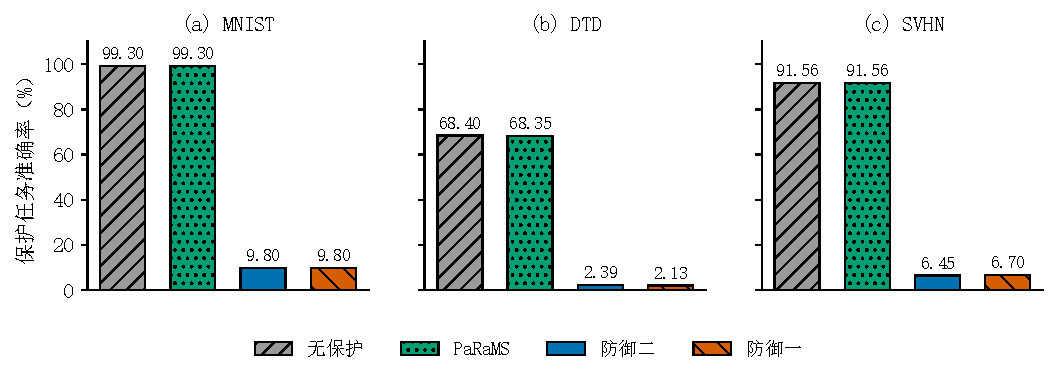
\includegraphics[width=.97\linewidth]{figures/aga_comparison.pdf}
\caption{原版AGA仅恢复保护专家后，三个保护任务的融合准确率。较低的融合准确率对应较强的保护效果。图中均为固定模型结果，不绘制独立重复实验的误差条。}
\label{fig:main}
\end{figure}

\clearpage
\section{防御二：基于任务子空间的全网络通道置换}
本方法改变视觉网络中768个残差通道的顺序，并同步修改各层相连参数。这里的通道是中间特征的坐标，不是类别、Attention头或MLP隐藏单元。\textbf{任务SVD用来选择交换哪些通道；全网络同步置换用来保持原模型的计算。}

\subsection{先用任务方向选择通道交换}
对任务矩阵$\Delta W_l=W_l-W_{0,l}$做SVD，其中$W_l$和$W_{0,l}$分别为专家与基座参数；取前32个右奇异方向$V_{l,32}$。范围为12个Transformer块的Q、K、V、Attention输出、MLP输入和输出，以及输入映射和视觉投影，共74个矩阵。设共同排列为$P$，实际矩阵改动为$E_l(P)$，计算
\begin{align}
T(P)&=\sum_l\frac{\norm{E_l(P)}_F^2}{\norm{W_l}_F^2},&
I(P)&=\sum_l\frac{\norm{E_l(P)V_{l,32}}_F^2}{\norm{W_l}_F^2},\\
F(P)&=\underbrace{[T(P)-I(P)]}_{\text{任务方向外的变化}}-\underbrace{I(P)}_{\text{任务方向内的变化}}.
\end{align}
目标是增大方向外的变化、减小方向内的变化。从原顺序开始，每次在未交换的通道中，选使$F$增加最多的一对；增量大于$10^{-10}$才接受，最多384对，相同增量按编号决定。三个主模型均固定384对，不用图片或分类成绩选择。这是贪心构造，不保证全局最优。

\subsection{再同步修改全网相连参数}
以列向量表示通道：Q、K、V和MLP输入矩阵改为$WP^{\mathsf T}$，Attention输出和MLP输出矩阵改为$PW$；输入映射、对应偏置、嵌入和LayerNorm参数也按同一顺序调整，最终投影还原输出坐标。因此
\begin{equation}
(WP^{\mathsf T})(Ph)=Wh.
\end{equation}
例如把第1、3通道互换，就同时互换下一矩阵的第1、3列（图\ref{fig:construction}）。残差两支使用同一排列，LayerNorm和逐元素非线性也保持对应，逐层计算由此保持。\textbf{独立功能保持来自这种配套修改，而不是假定SVD方向外没有功能作用。}完整FP32测试中，三个任务的全部预测均与原专家一致。

\begin{figure}[H]
\centering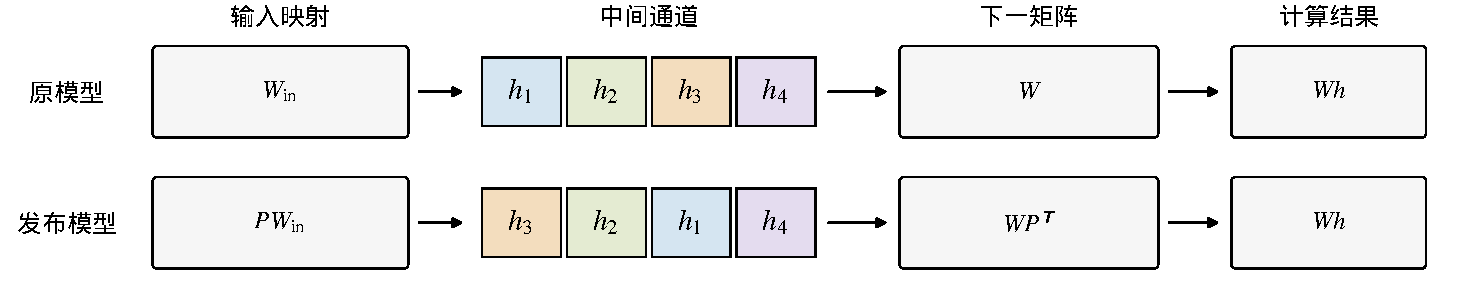
\includegraphics[width=.98\linewidth]{figures/construction.pdf}
\caption{一次通道交换的示意。输入映射与后续矩阵同时调整，右端计算结果保持。实际模型对全网络使用同一排列，而非只修改图中的两个矩阵。}
\label{fig:construction}
\end{figure}

\subsection{融合后，原来的对应关系被打乱}
伙伴保留自己的通道顺序。以输入映射为例，TA将$PW_e$与$W_p$按位置平均，得到$(PW_e+W_p)/2$；后续矩阵也分别平均，两端原有的配套关系因而不再自动成立。原版AGA处理Attention和MLP，没有完成全网共同排列的恢复。下一页报告实际分类结果，保护强度由这些结果检验。

\clearpage
\section{主实验结果}
表\ref{tab:main}在相同设置下比较无保护、PaRaMS、防御二和防御一，同时保留保护任务与伙伴任务准确率。防御二在三个任务上均保持原独立准确率；直接融合和原版AGA恢复后的保护任务准确率明显下降。PaRaMS在直接融合时有效，但原版AGA能使其融合性能回到接近无保护的水平。
\reporttablemain

除上述组合外，同一三份防御二发布模型还完成了其余伙伴组合的评价，没有因伙伴改变而重新构造保护参数。
\reporttablecross

\clearpage
\section{任务方向与修改幅度的作用}
\subsection{去掉任务方向项}
消融保持相同矩阵范围、奇异方向数、贪心规则和交换数量，只将目标从$T-2I$改为仅最大化$T$。两种顺序都已固定，表\ref{tab:ablation}保留全部结果。
\reporttableablation
相较于仅距离目标，加入任务方向后，三个任务的任务方向内平方改动分别减少16.83\%、17.69\%和18.27\%。原版AGA仅恢复保护专家时，MNIST和SVHN的融合准确率分别再降低1.47和2.07个百分点；DTD则高0.37个百分点。任务方向项确实影响了参数选择，但分类收益没有在三个任务上一致出现，不能将全部保护效果归因于SVD项。

\subsection{固定顺序下增加交换数量}
采用同一顺序的前96、192和384对交换，比较不同修改幅度。全部档位的完整MNIST独立准确率均为99.69\%，测试预测不变。
\begin{figure}[H]
\centering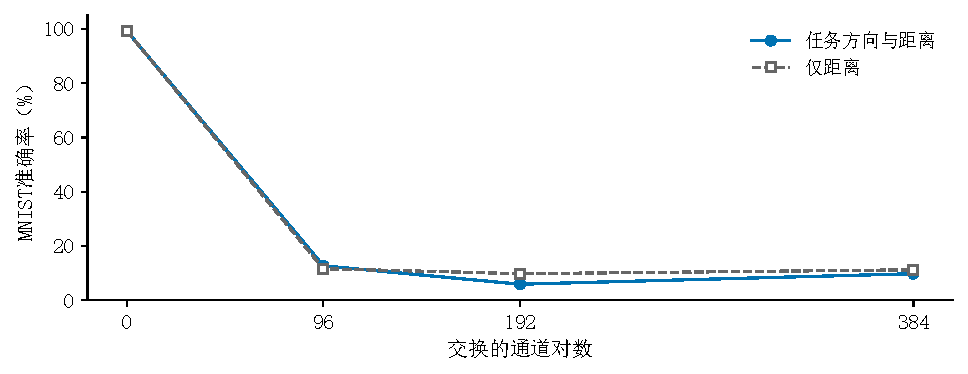
\includegraphics[width=.87\linewidth]{figures/extent.pdf}
\caption{MNIST保护、SVHN伙伴，TA系数0.5，原版AGA仅恢复保护专家。横轴只改变同一固定顺序的交换数量；0表示无保护。所有档位单独使用时的准确率均保持。}
\label{fig:extent}
\end{figure}
任务方向构造在96、192、384对交换时，原版AGA后的目标准确率分别为12.70\%、5.93\%和9.80\%。增加参数改动不带来单调增强的保护。主实验继续使用原先固定的384对模型，192对仅作为消融结果，不据此更换主模型。

\clearpage
\section{防御一：视觉投影零空间中的偏置扰动}
\subsection{构造及作用位置}
设最终LayerNorm输出为行向量，视觉投影为$P_e$。最终未归一化视觉特征为
\begin{equation}
t(h)=\left(\gamma_e\odot\frac{h-\mu(h)}{\sigma(h)}+\beta_e\right)P_e.
\end{equation}
只修改偏置$\beta_e$，取扰动$\delta$满足
\begin{equation}
\widetilde\beta_e=\beta_e+\delta,\qquad\delta P_e=0.
\end{equation}
因此独立模型的视觉特征在实数计算下保持。CLIP ViT-B/32的投影由768维到512维，提供非平凡零空间；实际按SVD数值秩确定。

实现先由$P_e$求零空间基，再利用目标专家与公开基座的固定插值模型确定扰动方向，以目标任务固定校准记录确定幅度。随后保存唯一偏置参数。除该偏置外，其他专家参数不变；不重新训练专家，不读取真实伙伴，也不按测试结果修改幅度。这是有结构限制的加性扰动，不是给任意参数加入独立噪声。

双专家TA系数为0.5时，最终投影同时变为$P_{\mathrm m}=(P_e+P_p)/2$。相较于未保护融合模型，偏置扰动的额外特征项为
\begin{equation}
\frac12\delta P_{\mathrm m}=\frac14\delta P_p.
\end{equation}
它不再由$\delta P_e=0$消去。表\ref{tab:main}中，三个任务独立准确率保持，原版AGA后的保护任务准确率为9.80\%、2.13\%和6.70\%。原版AGA没有修改最终LayerNorm偏置，因此这部分扰动被保留。

\subsection{其他融合方法的补充结果}
\reporttablesupplement
防御一在TA、TIES、DARE+TA及当前ProDistill适配下均降低了目标融合准确率。NUFILT的当前实现不合并被修改的最终偏置，两种顺序均未保留这一防御作用。此处区分融合规则和恢复攻击，不把不同融合算法计为新的攻击种类。

\clearpage
\section{八专家实验与结果范围}
八个参与专家按SUN397、Cars、RESISC45、EuroSAT、SVHN、GTSRB、MNIST、DTD的固定顺序、TA系数0.2合并。使用同一三份防御二发布模型，原版AGA只恢复保护专家，没有重新选择排列或参数。
\reporttableeight
八专家参与时，防御二在已评价的三个任务上仍降低了原版AGA后的目标准确率。该设置同时改变专家数量和融合系数，不能把差异全部解释为某一个因素。完整八数据集评价不在本表范围内。

\subsection{攻击者已知信息}
主结果对应不知道具体防御方式的原版AGA。若攻击者另外知道全网络通道置换这一修改方式，利用发布模型与公开基座进行输入映射匹配，可以还原当前防御二；无需原专家、秘密排列或图片。三个模型均已逐张量核对还原，恢复后的结果对应原专家的已有分数。防御一在已知最终偏置位置的清理操作下也可恢复。这些结果限定了当前方法的结论范围，不与原版AGA合并报告。

\subsection{实验完成情况与后续工作}
当前有效结果包括：三个任务的完整独立能力检查、双专家TA与原版AGA、六个保护方向、任务方向和幅度消融，以及八专家参与的三任务评价。主要记录已核对官方标签、逐类正确数、同一图片的预测变化，并用原128张批次上下文重放选定分数。相关模型、原始分数、源码版本及配置指纹均有保留，本次整理没有重新运行这些实验。

防御二目前通过参数置换保持原函数，任务SVD参与排列选择。进一步的核心工作是研究不依赖真实训练图的数值联合补偿：在任务方向少变的同时，扩大有功能作用的参数变化，并使这种补偿在融合后失效。现有数值探索尚不作为已完成的无数据方法列入主结果。后续优先完成这一构造及其必要验证。

\vspace{4pt}
\noindent\textbf{结果来源}\quad 本报告各表由项目统一实验表及其原始记录整理，另附同源Markdown表格和数值文件，可与原始实验记录核对。

\begin{thebibliography}{9}
\small
\bibitem{aga} Guo K, Zheng Q, Liang J, et al. On the Vulnerability of Parameter-Level Defenses to Model Merging. arXiv:2606.30360, 2026. \url{https://arxiv.org/abs/2606.30360}.
\bibitem{params} Wei J, Yu Z, Sakuma J. Disrupting Model Merging: A Parameter-Level Defense Without Sacrificing Accuracy. ICCV, 2025. \url{https://arxiv.org/abs/2503.07661}.
\bibitem{ta} Ilharco G, Ribeiro M T, Wortsman M, et al. Editing Models with Task Arithmetic. ICLR, 2023. \url{https://arxiv.org/abs/2212.04089}.
\end{thebibliography}
\end{document}
